\section{Stand der Forschung}


Die zunehmende Tendenz in Deutschland von bargeldloser Bezahlung erfordert neuen Umgang mit den 
eigegebenen Daten. Eine Studie von 2009 der Deutschen Bundesbank zeigte den rasanten Anstieg von 
bargeldloser Bezahlung in der Bundesrepublik seit der Einführung von solchen Zahlungsmethoden 
\cite{refrep:DBCP}.

\begin{figure}[htb]
    \centering{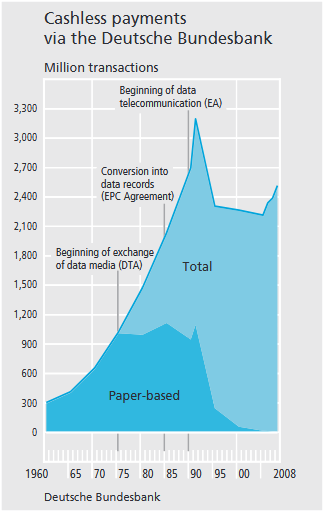
\includegraphics[width=5cm]{Bilder/refrep_DB.png}}
    \caption{Cashless payments via the Deutsche Bundesbank\\ (Bundesbank, 2009, S.52)}
    \label{fig:refrep_DB}
\end{figure}


Laut einer Statistik des Handelsforschungsinstituts EHI von 2019 \cite{refart:KSDL} bezahlen 48,6\% 
der deutschen ihre Waren mit Karte, wohingegen nur noch 46,9\% der deutschen den klassischen 
Weg über Bargeld gehen. Auch das kontaklose Bezahlen, bei dem kleine Beträge nicht einmal mit einer 
PIN bestätigt werden müssen, nimmt immer weiter zu. Doch gerade bei dieser Variante ist es sehr einfach
im Namen eines anderen zu bezahlen, was eine Sicherheitsrisiko darstellt. Diese Tendenz wurde auch
von \cite{refart:TDMP} in seiner Studie beobachtet, bei der er die meist verbreiteten Zahlungsarten
in verschidenen Regionen dieser Welt vergleicht. 


Immer wenn mit Karte bezahlt wird, gehen die Kunden davon aus, dass die Zahlungsabwicklung sicher ist. 
Wie sicher ist das bargeldlose Zahlen heutzutage wirklich? 


Aus diesem Grund ist Vertraulichkeit die erste und wichtigste Voraussetzung, das ein solches System 
erfüllen muss, um neue potenzielle Kunden zu gewinnen. 
Unter diesem Begriff Vertraulichkeit verstehen wir, dass es keine unautorisierte Informtionsgewinnung gibt (Quelle: Wendzel)
Unter diesem Begriff soll ein System nur auf 
autorisierte Informationen zugreifen \cite{refbook:SWIS}. In dieser Hinsicht ist die Entwicklung 
einer Click and Buy Maschine so zu konzipieren, dass sie einen sicheren Umgang mit den Kundendaten
anbietet. Diese Interaktion zwischen Kunde und systemkritischen Mechanismen wurde von \cite{refart:HARE}
so dargestellt:

\vfill
\begin{figure}[htb]
    \centering{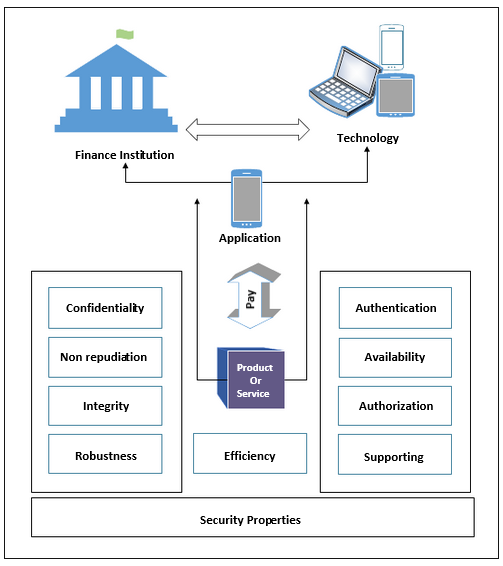
\includegraphics[width=5cm]{Bilder/refark_HARE.png}}
    \caption{Sicherheitseigenschaften von digitalen Zahlungsmethode (Hassan et al. 2020, S8)}
    \label{fig:refark_HARE}
\end{figure}
\vfill

Zudem sollten die weiteren Schutzziele der IT-Sicherheit: Integrität, Verfügbarkeit und Authentizität
berücksichtigt werden, sodass die Systeme einwandfrei und sicher funktionieren \cite{refip:GMPS}. 
Eine Zahlungsmethode, bei der alle Vorraussetzungen erfüllt werden, kann in der Lage sein, das Vertrauen 
und die Akzeptanz von den Nutzenden zu bekommen \cite{refart:HARE}. Besonders im deutschen Markt, spielen
die oben genannten Schutzziele eine wesentliche Rolle \cite{refip:DKAM}, da sie ein Entscheidungsfaktor 
dafür sind, ob ein System genutzt wird oder nicht.


%\cite{inbook:MHNS} nennt solche Maschinen Cyber-Physical System (CPS), weil sie eine Interaktion zwischen 
%Nutzer und einem oder vielen Systemen darstellt. In dieser Zusammenarbeit spielt der Datenaustausch 
%eine wesentliche Rolle, besonders von der Seite des Nutzenden. Diese Technologie zielt eine günstigere 
%Entwicklung ab, ohne die Sicherheit zu vernachlässigen. Eine Interaktion is erfolgereich, 
%wenn die genannten Sicherheitszielle erfüllt wurden.


Da es um einen dynamischen und breiten Bereich geht, bei dem es sehr schnell zu Änderungen kommen kann, 
besonders bei den Angriffstechniken, müssen die dazu gehörige \cite{refip:NYRS} Technologie stets 
weiterentwickelt und angepasst werden, um Vertraulichkeitsverlust seitens der Kunden zu vermeiden. 
Da die Vertraulichkeit noch nicht zu 100 Prozent gewähleistet werden kann, verweigern viele Kunden
das bargeldlose Bezahlen.

Viele Studien befassen sich mit den verschiedenen Aspekten der Sicherheit bei bargeldlosen Zahlungsmethoden.
Die Literatur dieses Forschungsfeldes ist sehr umfangreich und kümmert sich um die Vielfältigkeit 
dieser heterogen \cite{refip:GMPS} Umgebung. Im nachfolgenden Artikel sollen zwei dieser Technologien 
in Bezug auf Angriffstechniken und Gegenmaßnahmen genauer betrachtet werden.





\textbf{\textcolor{red}{Ab hier können wir dann versuchen, die Informatien aus den Artikeln zu nehmen, solche
die du hier hinzugefügt hast und solche, die ich dir am Fr schickte}}

\vspace{2cm}
\textbf{Ich würde diesen Satz in den nächsten Kapitel verwenden und erweitern mit unseren Recherchen, damit wird 
die Literatur rechtfertigen können}
Um das zu bewerkstelligen, ist der aktuelle technische Stand von entscheidener Bedeutung. 
Ausgehend von dieser Informationen muss das Glasfasernetz eventuell erweitert oder auch neu verlegt werden.
Denn das Ziel ist es, technisch gesehen auf dem neusten Stand zu sein, damit das Click and Buy System für die Zukunft abgesichert ist.
Außerdem wird durch den Ausbau des Glasfasernetzes die Region insgesamt deutlich attraktiver gemacht, was vielleicht auch Menschen dazu bringt
in diese Region zu ziehen. Denn jedem ist klar, dass ein guter Internetausbau essentiell ist, um vielleicht auch mal von zuhause aus zu arbeiten.